\documentclass[12pt]{article}
\usepackage[margin=0.75in]{geometry}
\usepackage{float}
\usepackage{multicol}
\usepackage{lmodern}
\usepackage{amssymb,amsmath}
\usepackage{ifxetex,ifluatex}
\usepackage{fixltx2e} % provides \textsubscript
\ifnum 0\ifxetex 1\fi\ifluatex 1\fi=0 % if pdftex
  \usepackage[T1]{fontenc}
  \usepackage[utf8]{inputenc}
\else % if luatex or xelatex
  \ifxetex
    \usepackage{mathspec}
    \usepackage{xltxtra,xunicode}
  \else
    \usepackage{fontspec}
  \fi
  \defaultfontfeatures{Mapping=tex-text,Scale=MatchLowercase}
  \newcommand{\euro}{€}
\fi
% use upquote if available, for straight quotes in verbatim environments
\IfFileExists{upquote.sty}{\usepackage{upquote}}{}
% use microtype if available
\IfFileExists{microtype.sty}{%
\usepackage{microtype}
\UseMicrotypeSet[protrusion]{basicmath} % disable protrusion for tt fonts
}{}
\usepackage{longtable,booktabs}
\usepackage{graphicx}
\makeatletter
\def\maxwidth{\ifdim\Gin@nat@width>\linewidth\linewidth\else\Gin@nat@width\fi}
\def\maxheight{\ifdim\Gin@nat@height>\textheight\textheight\else\Gin@nat@height\fi}
\makeatother
% Scale images if necessary, so that they will not overflow the page
% margins by default, and it is still possible to overwrite the defaults
% using explicit options in \includegraphics[width=3.5in][width, height, ...]{}
\setkeys{Gin}{width=\maxwidth,height=\maxheight,keepaspectratio}
\ifxetex
  \usepackage[setpagesize=false, % page size defined by xetex
              unicode=false, % unicode breaks when used with xetex
              xetex]{hyperref}
\else
  \usepackage[unicode=true]{hyperref}
\fi
\hypersetup{breaklinks=true,
            bookmarks=true,
            pdfauthor={Brandon LeBeau},
            pdftitle={PSQF 4143: Section 6},
            colorlinks=true,
            citecolor=blue,
            urlcolor=blue,
            linkcolor=magenta,
            pdfborder={0 0 0}}
\urlstyle{same}  % don't use monospace font for urls
\setlength{\parindent}{0pt}
\setlength{\parskip}{6pt plus 2pt minus 1pt}
\setlength{\emergencystretch}{3em}  % prevent overfull lines
\setcounter{secnumdepth}{0}

\title{PSQF 4143: Section 6}
\author{Brandon LeBeau}
\date{}

\begin{document}
\maketitle

\section{Descriptive vs Inferential
Statistics}\label{descriptive-vs-inferential-statistics}

\begin{itemize}
\itemsep1pt\parskip0pt\parsep0pt
\item
  Descriptive:

  \begin{itemize}
  \itemsep1pt\parskip0pt\parsep0pt
  \item
    Useful if we are interested in a single group or comparison
  \item
    Major interest is only with the subjects on hand
  \end{itemize}
\item
  Inferential:

  \begin{itemize}
  \itemsep1pt\parskip0pt\parsep0pt
  \item
    Useful whenever we are interested in a larger group of subjects than
    just those on hand
  \item
    Gallup poll is the most common example
  \end{itemize}
\end{itemize}

\section{Inferential Loop}\label{inferential-loop}

\begin{enumerate}
\def\labelenumi{\arabic{enumi}.}
\itemsep1pt\parskip0pt\parsep0pt
\item
  Ask a question
\item
  Draw a sample from the population
\item
  Analyze Data
\item
  Make inference
\end{enumerate}

\begin{itemize}
\itemsep1pt\parskip0pt\parsep0pt
\item
  What happens if we draw a second sample?

  \begin{itemize}
  \itemsep1pt\parskip0pt\parsep0pt
  \item
    Would we have the same result?
  \end{itemize}
\end{itemize}

\section{Reasons for Sampling}\label{reasons-for-sampling}

\begin{itemize}
\itemsep1pt\parskip0pt\parsep0pt
\item
  Not all of the population is accessible

  \begin{itemize}
  \itemsep1pt\parskip0pt\parsep0pt
  \item
    Too expensive
  \item
    Physically or practically impossible to survey the entire population
  \end{itemize}
\item
  Data collection procedure consumes the elements of the population

  \begin{itemize}
  \itemsep1pt\parskip0pt\parsep0pt
  \item
    wine tasting, missle testing, rocket launches
  \end{itemize}
\end{itemize}

\section{Sampling example}\label{sampling-example}

\begin{figure}[H]
\centering
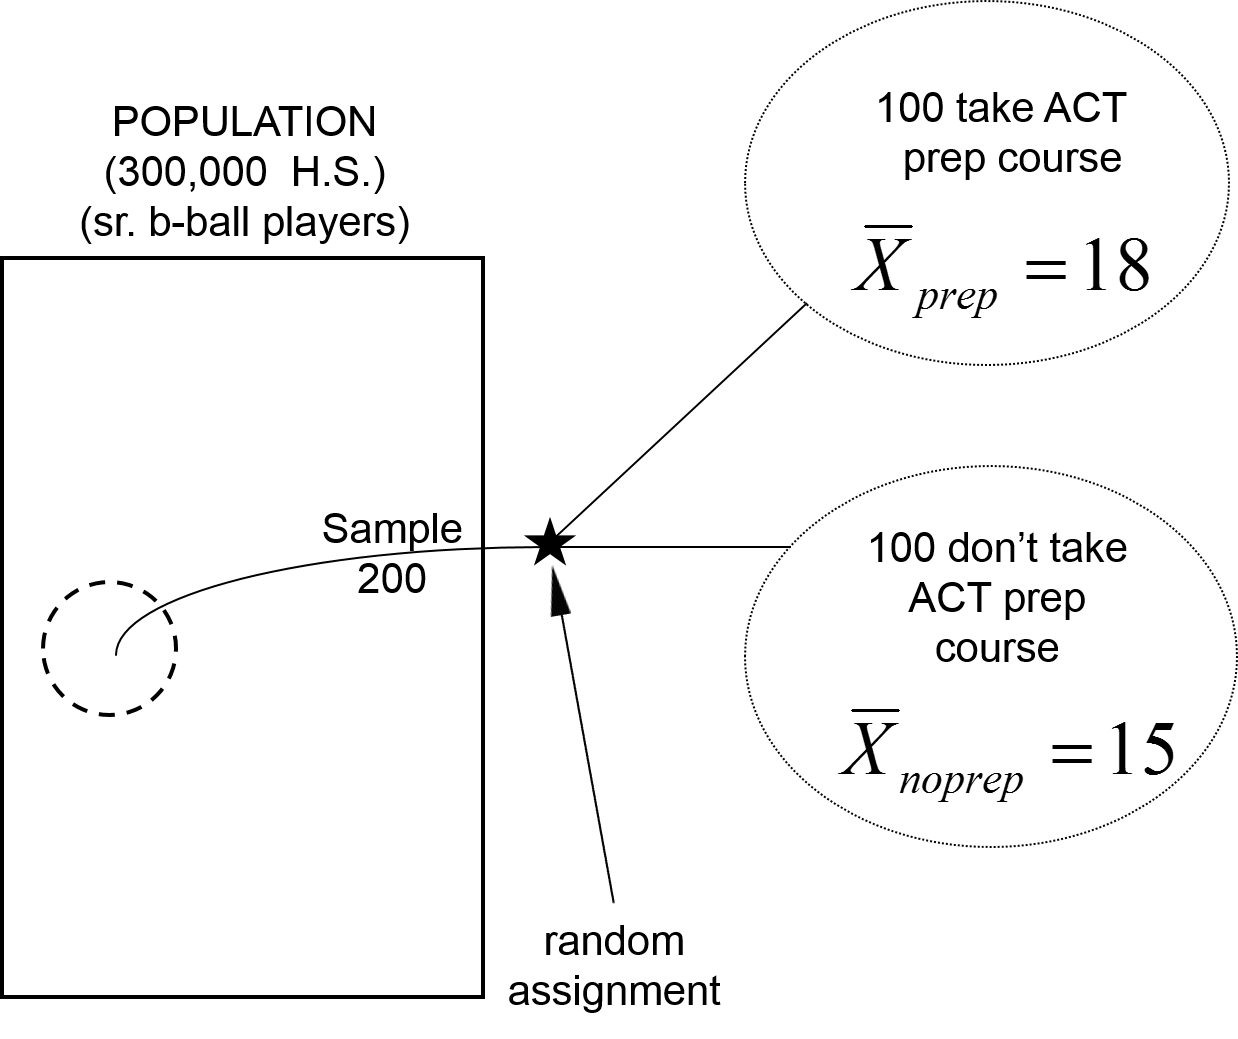
\includegraphics[width=3.5in]{sample_examp.png}
\caption{}
\end{figure}

\begin{itemize}
\itemsep1pt\parskip0pt\parsep0pt
\item
  Would the mean score of all 300,000 be 18 if they all took the prep
  course?
\item
  Would the mean score of all 300,000 be 15 if they did not take the
  prep course?

  \begin{itemize}
  \itemsep1pt\parskip0pt\parsep0pt
  \item
    Both samples contain error.
  \item
    Therefore, it is not sufficient to consider just the observed
    difference.
  \item
    Rather, we need a probability statement to quantify the error.
  \end{itemize}
\item
  How to do that?

  \begin{itemize}
  \itemsep1pt\parskip0pt\parsep0pt
  \item
    We might assume that there is no difference between the two groups.
  \item
    Based on this assumption, we then determine the probability that the
    difference between the means is equal to 3.
  \item
    If this probability is small, then maybe our assumption was wrong.
  \end{itemize}
\item
  Probability is the basis of inferential statistics.
\end{itemize}

\section{Three Characteristics of an
Experiment}\label{three-characteristics-of-an-experiment}

\begin{enumerate}
\def\labelenumi{\arabic{enumi}.}
\itemsep1pt\parskip0pt\parsep0pt
\item
  Repeatable
\item
  Uncertainty of outcome
\item
  Able to specify all possible outcomes
\end{enumerate}

\begin{itemize}
\itemsep1pt\parskip0pt\parsep0pt
\item
  Example:

  \begin{itemize}
  \itemsep1pt\parskip0pt\parsep0pt
  \item
    Rolling a six-sided die

    \begin{enumerate}
    \def\labelenumi{\arabic{enumi}.}
    \itemsep1pt\parskip0pt\parsep0pt
    \item
      You can roll the die over and over again
    \item
      On any given roll, you don't know ahead of time which number will
      come up.
    \item
      The outcome on any given roll will be 1 or 2 or 3 or 4 or 5 or 6.
    \end{enumerate}
  \end{itemize}
\end{itemize}

\section{Definitions}\label{definitions}

\begin{itemize}
\itemsep1pt\parskip0pt\parsep0pt
\item
  An \textbf{event} is an observable outcome
\item
  A \textbf{generating event} is any repeatable process that results in
  only one outcome at a time

  \begin{itemize}
  \itemsep1pt\parskip0pt\parsep0pt
  \item
    Examples: Flipping a coin, rolling a die, drawing a card
  \end{itemize}
\item
  The \textbf{probability (Pr)} of an event is the relative frequency
  with which that event would be observed over an infinite number of
  repetitions of the generating event, when each repetition is conducted
  in a like manner.
\end{itemize}

\section{Probability of an Event}\label{probability-of-an-event}

\begin{itemize}
\item
  Example: Flipping a coin
  \[Pr(heads) = \frac{\mbox{number of heads observed}}{\mbox{total number of flips}}\]
  \[ = \frac{f(heads) }{N}\] when observations are recorded for an
  infinite number of flips
\item
  As a proportion, \(0 \leq Pr \leq 1\)
\item
  A probability is a proportion characterizing an infinitely long series
  of occurrences

  \begin{itemize}
  \itemsep1pt\parskip0pt\parsep0pt
  \item
    It does not tell us precisely what would happen over any short run
  \end{itemize}
\item
  We could flip a coin several thousand times to obtain an
  \textbf{estimate} of the true proportion of heads

  \begin{itemize}
  \itemsep1pt\parskip0pt\parsep0pt
  \item
    This kind of estimate is called an \emph{empirical probability}
  \end{itemize}
\end{itemize}

\section{More Definitions}\label{more-definitions}

\begin{itemize}
\itemsep1pt\parskip0pt\parsep0pt
\item
  A \textbf{sample space (S)} is a set of all possible outcomes of an
  experiment (generating event)
\item
  Each individual outcome in a sample space is called a **sample point*
  \((s_{j})\)
\item
  Given a sample space, S, consisting of n sample points, \(s_{j}\)

  \begin{itemize}
  \itemsep1pt\parskip0pt\parsep0pt
  \item
    Let \(Pr(s_{j}) \geq 0\) be paired with each sample point
  \item
    Then \(\sum Pr(s_{j}) = 1\)
  \end{itemize}
\end{itemize}

\section{Example}\label{example}

\begin{itemize}
\item
  Example: Rolling a fair, six-sided die \[S = {1, 2, 3, 4, 5, 6}\]
  \[Pr(1) = Pr(2) = Pr(3) = Pr(4) = Pr(5) = Pr(6) = 1/6\]
  \[Pr(s_{1}) = Pr(s_{2}) = Pr(s_{3}) = Pr(s_{4}) = Pr(s_{5}) = Pr(s_{6}) = 1/6\]
  \[\sum Pr(s_{j}) = \frac{1}{6} + \frac{1}{6} + \frac{1}{6} + \frac{1}{6} + \frac{1}{6} + \frac{1}{6} = 1\]
\item
  Equally Likely Model:

  \begin{itemize}
  \itemsep1pt\parskip0pt\parsep0pt
  \item
    Given a sample space S with n sample points:
    \(S = {s_{1}, s_{2}, \ldots, s_{n}}\)
  \item
    If \(Pr(s_{n}) = 1/n\) for each sample point
  \item
    Then the outcomes are equally likely
  \end{itemize}
\end{itemize}

\section{Probability}\label{probability}

\begin{itemize}
\itemsep1pt\parskip0pt\parsep0pt
\item
  Given a population of possible outcomes (that is, a sample space),
  each of which is equally likely, the \textbf{probability of event A}
  on a single trial is equal to the number of possible outcomes yielding
  A divided by the total number of possible outcomes
\end{itemize}

\[Pr(A) = \frac{\mbox{# of ways A can occur}}{\mbox{total # of possible outcomes}}\]

\section{Probability 2}\label{probability-2}

\begin{itemize}
\item
  Let the set of sample points in the sample space of an experiment be
  \(s_{j}(j = 1, 2, 3, \ldots, n)\) and let the respective probability
  values assigned to these events be represented by \(Pr(s_{j})\)
\item
  Then the set of pairs \({[sj , Pr(s_{j})]; j = 1, 2, 3, \ldots, n}\)
  is the probability distribution of the experiment
\item
  Example: Rolling a fair, six-sided die
\end{itemize}

\begin{longtable}[c]{@{}cc@{}}
\toprule
\(s_{j}\) & \(Pr(s_{j})\)\tabularnewline
\midrule
\endhead
1 & 1/6\tabularnewline
2 & 1/6\tabularnewline
3 & 1/6\tabularnewline
4 & 1/6\tabularnewline
5 & 1/6\tabularnewline
6 & 1/6\tabularnewline
\bottomrule
\end{longtable}

\begin{figure}[H]
\centering
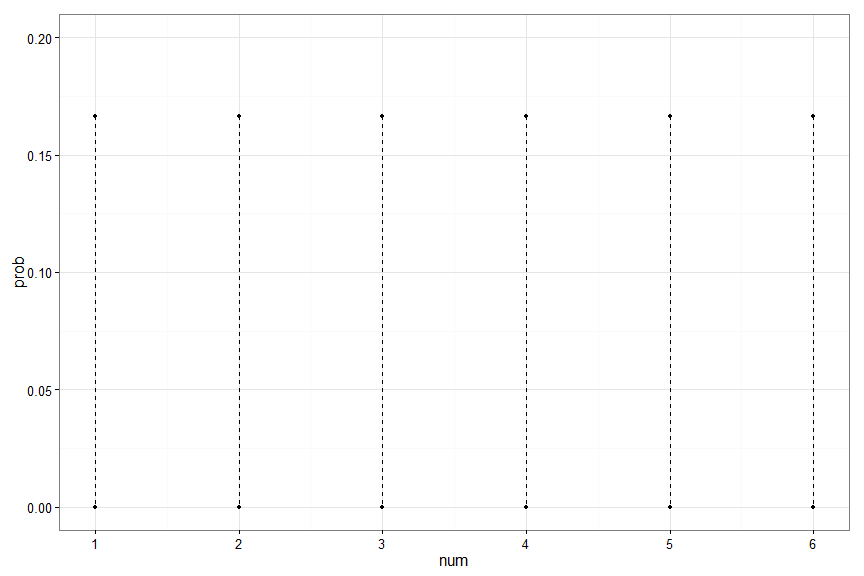
\includegraphics[width=3.5in]{figure/probdie-1.png}
\caption{plot of chunk probdie}
\end{figure}

\section{Two Ways to Calculate
Probability}\label{two-ways-to-calculate-probability}

\begin{enumerate}
\def\labelenumi{\arabic{enumi}.}
\itemsep1pt\parskip0pt\parsep0pt
\item
  Actually conduct the experiment a large number of times

  \begin{itemize}
  \itemsep1pt\parskip0pt\parsep0pt
  \item
    This is called an empirical or Monte Carlo method
  \end{itemize}
\item
  Use a theoretical probability model (for example, the equally likely
  model)

  \begin{itemize}
  \itemsep1pt\parskip0pt\parsep0pt
  \item
    With this method, you do not have to conduct even a single trial of
    the experiment
  \end{itemize}
\end{enumerate}

\section{Coin Once}\label{coin-once}

\begin{figure}[H]
\centering
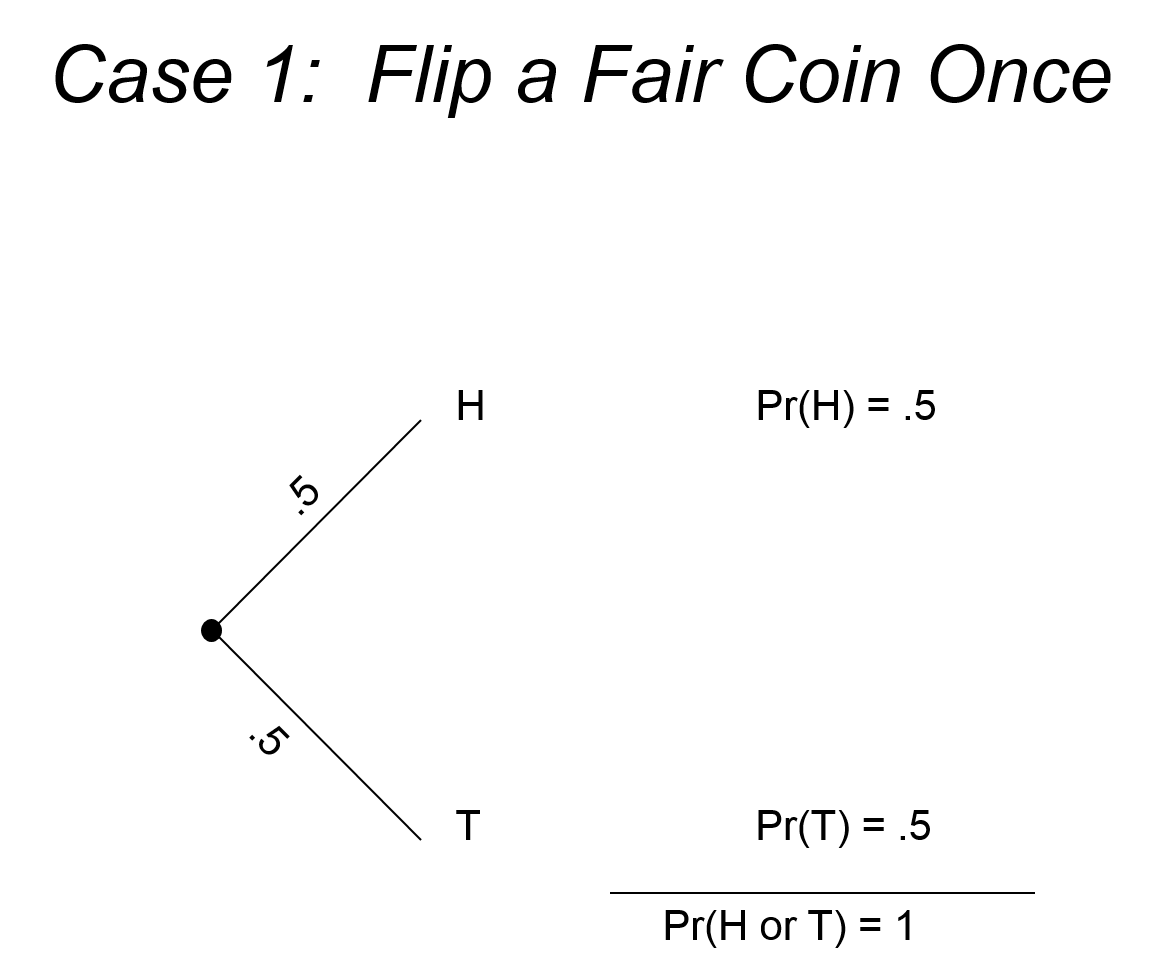
\includegraphics[width=3.5in]{coin_once.png}
\caption{Flip Coin Once}
\end{figure}

\section{Addition Theorem (OR Rule)}\label{addition-theorem-or-rule}

\begin{itemize}
\itemsep1pt\parskip0pt\parsep0pt
\item
  The probability of occurrence of any one of several particular events
  is the sum of their individual probabilities, provided the events are
  mutually exclusive (that is, the occurrence of one precludes others)
\item
  To find the chance that at least one of two things will happen, check
  to see if they are mutually exclusive; if they are, add their
  probabilities
\item
  \(Pr(A or B) = Pr(A) + Pr(B)\), provided A and B are mutually
  exclusive
\end{itemize}

\section{Coin Twice}\label{coin-twice}

\begin{figure}[H]
\centering
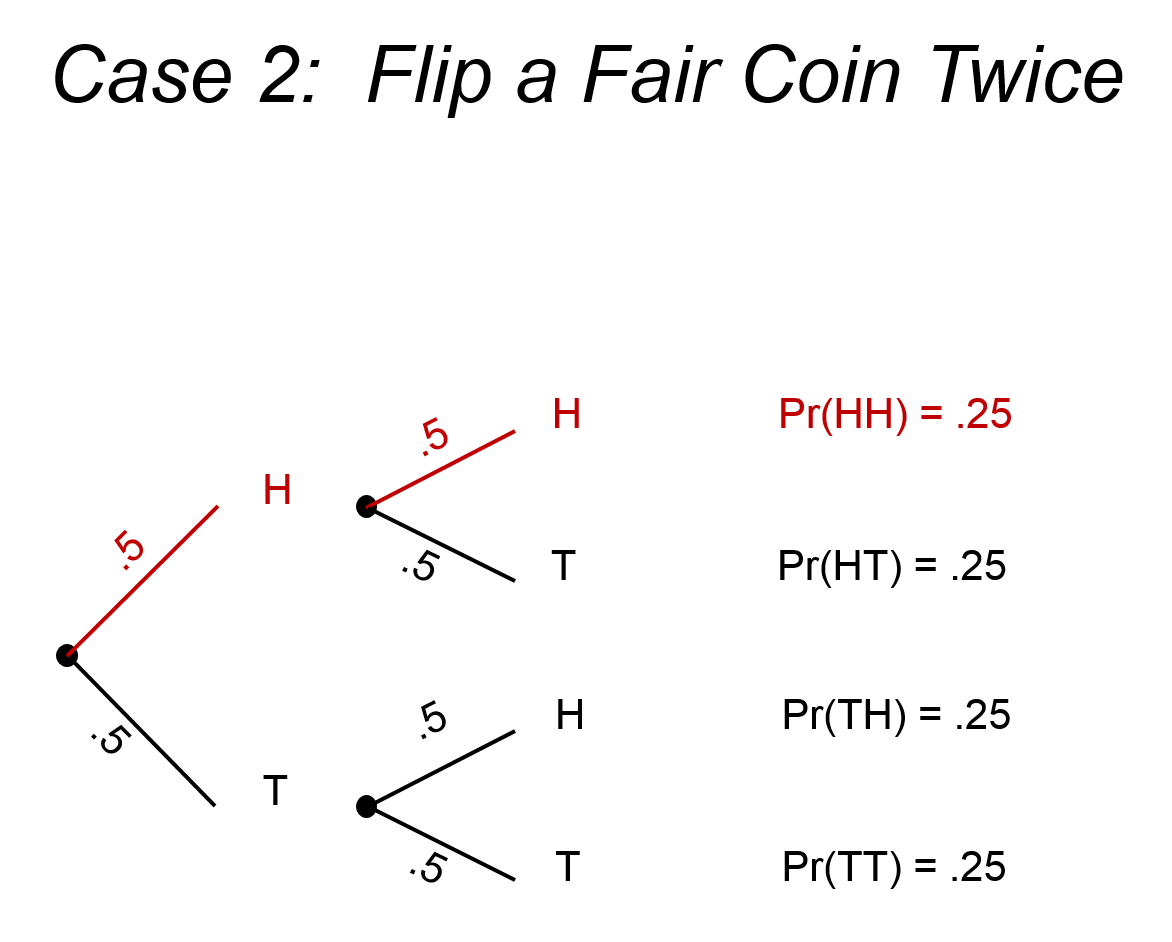
\includegraphics[width=3.5in]{coin_twice.png}
\caption{Flip Coin Twice}
\end{figure}

\section{Multiplication Theorem (AND
Rule)}\label{multiplication-theorem-and-rule}

\begin{itemize}
\itemsep1pt\parskip0pt\parsep0pt
\item
  Given two events, A and B, the probability of obtaining both A and B
  jointly (or successively) is the product of their separate
  probabilities

  \begin{itemize}
  \itemsep1pt\parskip0pt\parsep0pt
  \item
    if A and B are independent (that is, the outcome of one event has no
    influence on, and is in no way related to, the outcome of the other)
  \item
    then \(Pr(A and B) = Pr(A) * Pr(B)\)
  \end{itemize}
\item
  if A and B are not independent

  \begin{itemize}
  \itemsep1pt\parskip0pt\parsep0pt
  \item
    then \(Pr(A and B) = Pr(A) × Pr(B|A)\)
  \item
    or \(Pr(A and B)= Pr(B) * Pr(A|B)\)
  \end{itemize}
\end{itemize}

\section{Coin Thrice}\label{coin-thrice}

\begin{figure}[H]
\centering
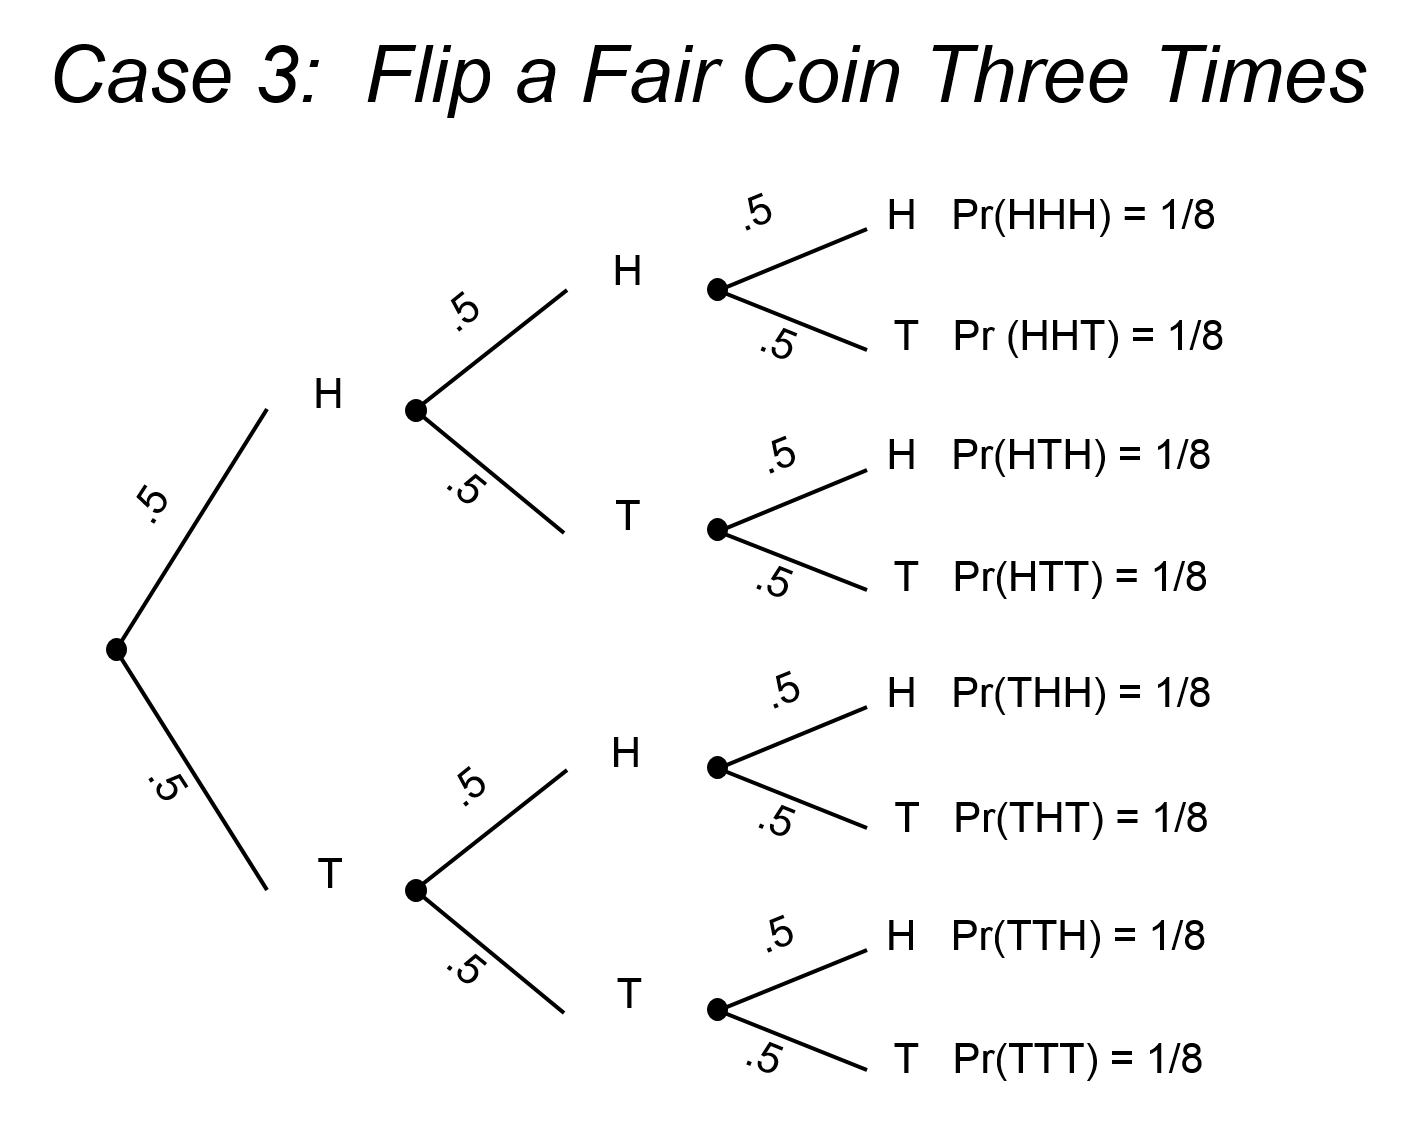
\includegraphics[width=3.5in]{coin_three.png}
\caption{Flip Coin Thrice}
\end{figure}

\section{Binomial Experiment}\label{binomial-experiment}

\begin{itemize}
\itemsep1pt\parskip0pt\parsep0pt
\item
  Characteristics:

  \begin{enumerate}
  \def\labelenumi{\arabic{enumi}.}
  \itemsep1pt\parskip0pt\parsep0pt
  \item
    Universe of N object of two kinds, A or \(\bar{A}\) (not A)
  \item
    Randomly select an object from this universe, note its type, and
    replace it

    \begin{itemize}
    \itemsep1pt\parskip0pt\parsep0pt
    \item
      Sampling with replacement
    \end{itemize}
  \item
    The probability of an A-type object in the universe it \(\phi\)
    (that is, \(Pr(A) = \phi\) and \(Pr(\bar{A}) = 1 - \phi\)).
  \item
    Pr(A) must remain constant over n repetitions of the selection
    process.
  \item
    The outcome of interest is a random variable
  \end{enumerate}
\item
  Binomial Exansion

  \begin{itemize}
  \itemsep1pt\parskip0pt\parsep0pt
  \item
    Given a binomial experiment, the probability value associated with
    each possible outcome can be found using the binomial expansion
    \[ (P + Q)^N\]
  \item
    P is the probability of the outcome (event) of interst
  \item
    Q is the probability of the other outcome (event); that is,
    \(Q = 1 - P\)
  \item
    N is the number of trials
  \end{itemize}
\end{itemize}

\section{Binomial Expansion Example}\label{binomial-expansion-example}

\begin{itemize}
\itemsep1pt\parskip0pt\parsep0pt
\item
  Flip a fair coin twice:

  \begin{itemize}
  \itemsep1pt\parskip0pt\parsep0pt
  \item
    \(P = 0.5\)
  \item
    \(Q = 0.5\)
  \item
    \(N = 2\) \[(P + Q)^N = (P + Q)^2 = P^2 + 2PQ + Q^2 \]
    \[ = (0.5)^2 + 2(0.5)(0.5) + (0.5)^2 \] \[ = 0.25 + 0.5 + 0.25 = 1\]
  \end{itemize}
\end{itemize}

\section{Probability Distribution}\label{probability-distribution}

\begin{figure}[H]
\centering
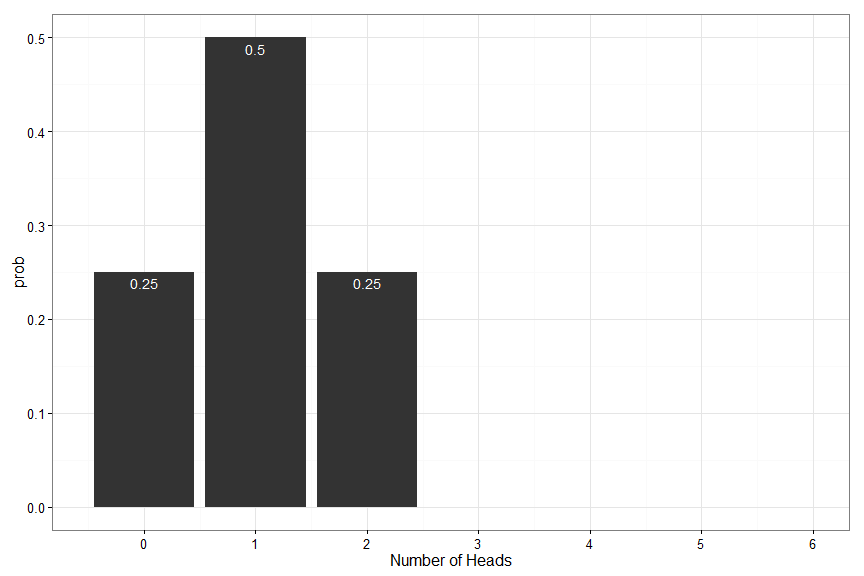
\includegraphics[width=3.5in]{figure/prob2heads-1.png}
\caption{plot of chunk prob2heads}
\end{figure}

\section{Binomial Expansion Example
2}\label{binomial-expansion-example-2}

\begin{itemize}
\itemsep1pt\parskip0pt\parsep0pt
\item
  Flip a fair coin thrice:

  \begin{itemize}
  \itemsep1pt\parskip0pt\parsep0pt
  \item
    \(P = 0.5\)
  \item
    \(Q = 0.5\)
  \item
    \(N = 3\) \[(P + Q)^N = (P + Q)^3 = P^3 + 3P^2Q + 3PQ^2 + Q^3 \]
    \[ = (0.5)^3 + 3(0.5)^2(0.5) + 3(0.5)(0.5)^2 + (0.5)^3 \]
    \[ = 0.125 + 0.375 + 0.375 + 0.125 = 1\]
  \end{itemize}
\end{itemize}

\section{Probability Distribution 2}\label{probability-distribution-2}

\begin{figure}[H]
\centering
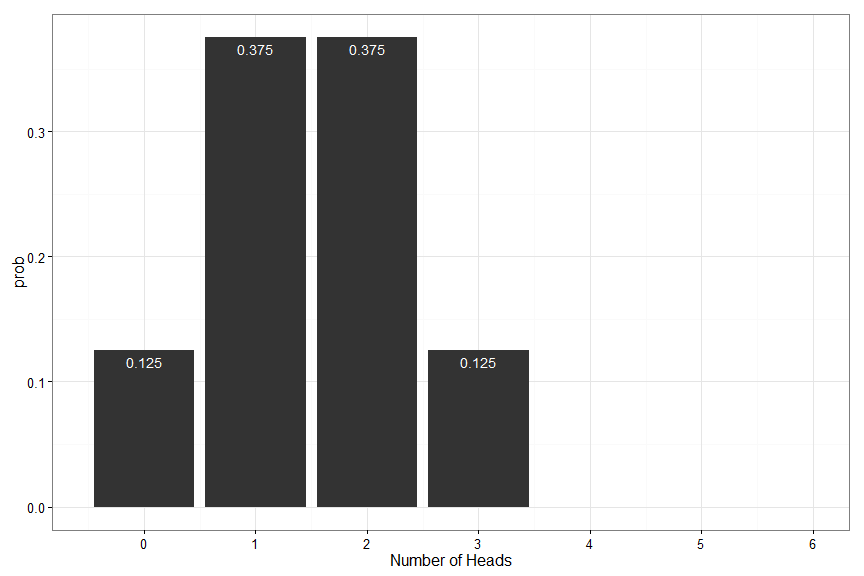
\includegraphics[width=3.5in]{figure/prob3heads-1.png}
\caption{plot of chunk prob3heads}
\end{figure}

\section{Binomial Expansion}\label{binomial-expansion}

\begin{itemize}
\itemsep1pt\parskip0pt\parsep0pt
\item
  Beyond this the math becomes more difficult
\item
  Fortunately there are tables for this.
\item
  The binomial table can be found in the course pack.
\item
  Example: Flip a coin five times
\end{itemize}

\section{Probability Distribution 3}\label{probability-distribution-3}

\begin{figure}[H]
\centering
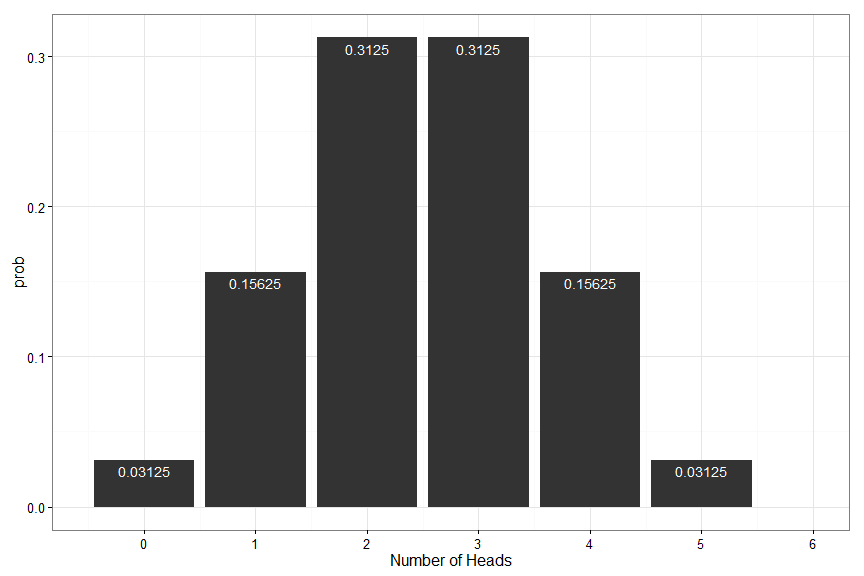
\includegraphics[width=3.5in]{figure/prob5heads-1.png}
\caption{plot of chunk prob5heads}
\end{figure}

\section{Characteristics of the Binomial
Distribution}\label{characteristics-of-the-binomial-distribution}

\begin{itemize}
\item
  Mean: \(N * P\)
\item
  Variance: \(N * P * (1 - P)\)
\item
  N is the number of trials
\item
  P is the Pr(success) on a given trial
\item
  Example: Number of heads in four flips of a fair coin

  \begin{itemize}
  \itemsep1pt\parskip0pt\parsep0pt
  \item
    \(N = 4\)
  \item
    \(P = 0.5\)
  \item
    Mean = 2
  \item
    Variance = 1
  \end{itemize}
\end{itemize}

\section{Probability Distribution
Example}\label{probability-distribution-example}

\begin{figure}[H]
\centering
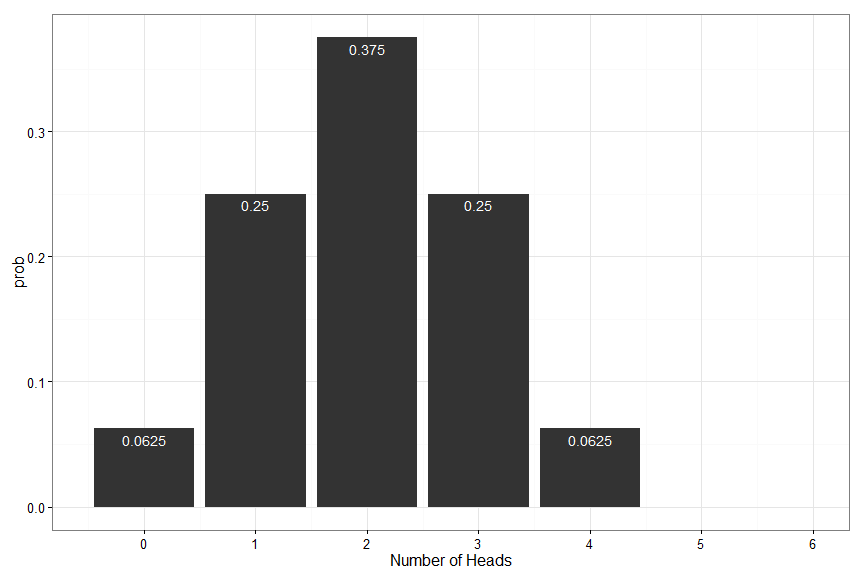
\includegraphics[width=3.5in]{figure/prob4heads-1.png}
\caption{plot of chunk prob4heads}
\end{figure}

\section{Normal Approximation to Binomial
Distribution}\label{normal-approximation-to-binomial-distribution}

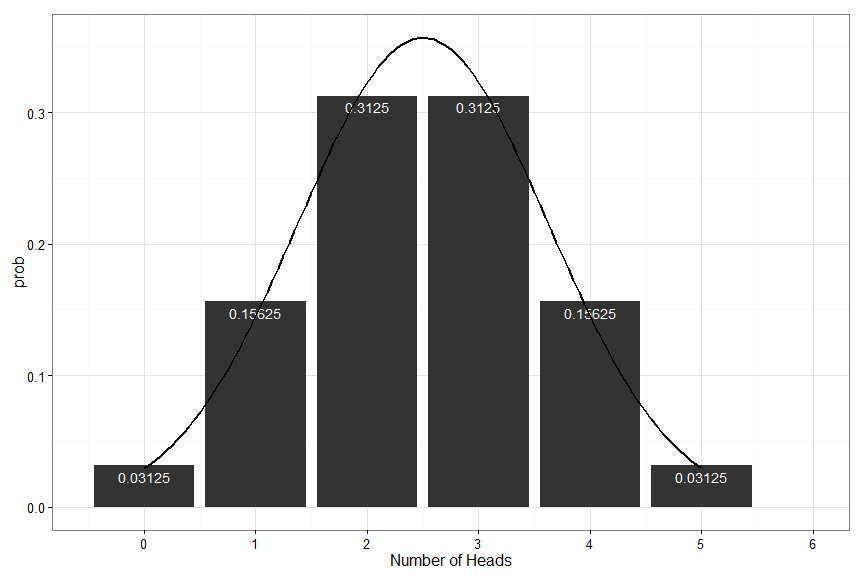
\includegraphics[width=3.5in]{figure/normapprox-1.png}
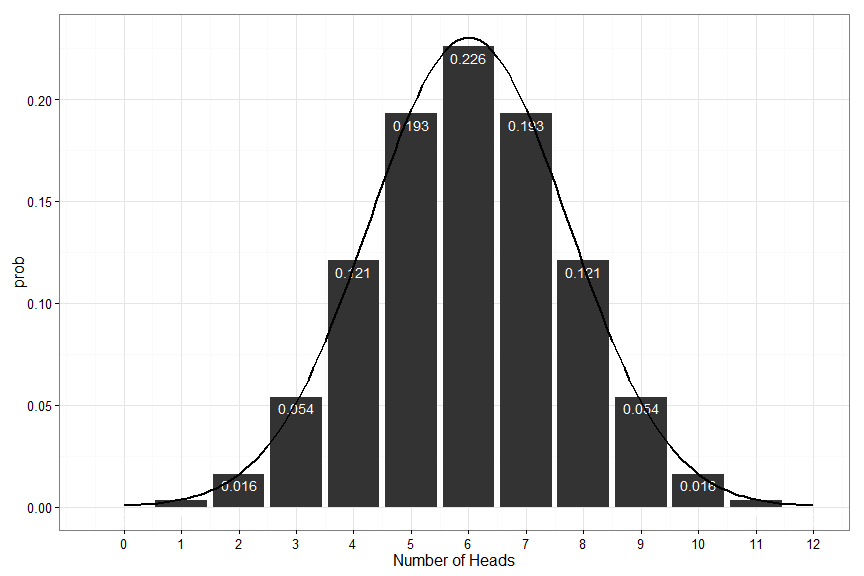
\includegraphics[width=3.5in]{figure/normapprox-2.png}

\section{Another Binomial Example}\label{another-binomial-example}

\begin{figure}[H]
\centering
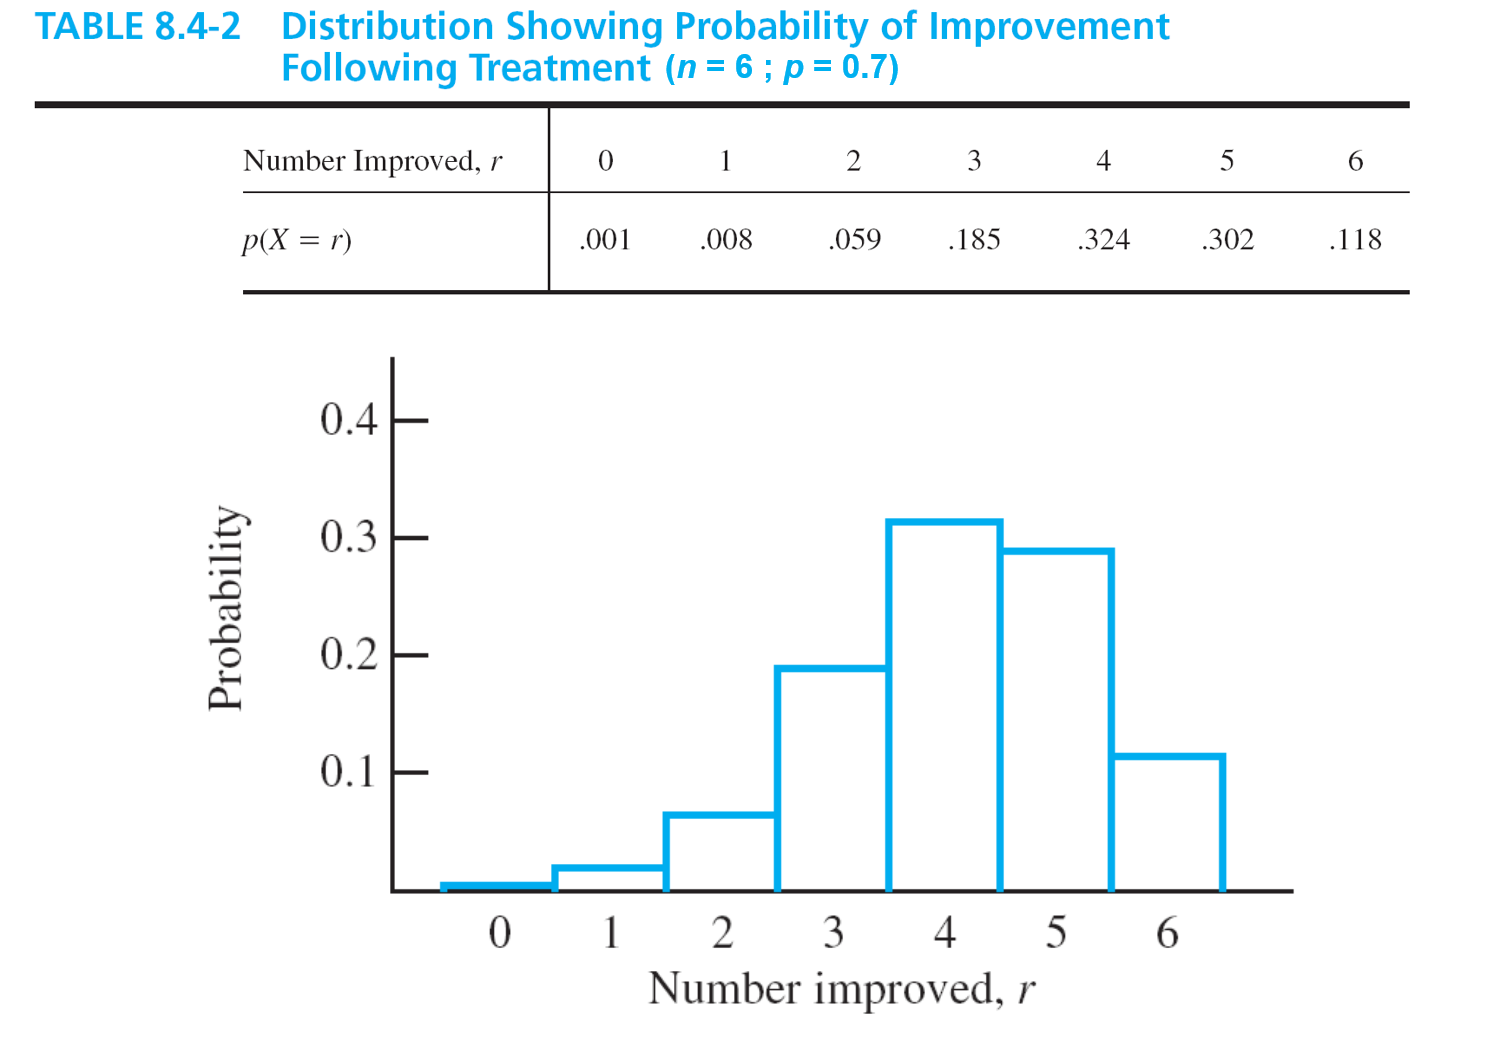
\includegraphics[width=3.5in]{binom_improve.png}
\caption{Binom Example 0.7}
\end{figure}

\section{Example 3}\label{example-3}

What is the chance that someone could get at least half of the questions
correct on a 10-question multiple-choice test (4 options per question)
if he/she was randomly guessing on each question?

\section{Taste Test}\label{taste-test}

\begin{itemize}
\itemsep1pt\parskip0pt\parsep0pt
\item
  Somebody claims to be able to taste the difference between Coke and
  Pepsi
\item
  To test this claim, we will conduct an experiment

  \begin{enumerate}
  \def\labelenumi{\arabic{enumi}.}
  \itemsep1pt\parskip0pt\parsep0pt
  \item
    Blindfold the individual
  \item
    Let the individual taste a sample of Coke and a sample of Pepsi in
    random order, then ask her to identify which is which
  \item
    Repeat Step 2 nine more times (10 replications altogether)
  \end{enumerate}
\item
  The number of correct identifications in 10 trials is the outcome of
  the experiment
\end{itemize}

\section{Taste Test Results}\label{taste-test-results}

\begin{itemize}
\itemsep1pt\parskip0pt\parsep0pt
\item
  Suppose she correctly identifies Coke 7 times in 10 trials.
\item
  Hypothesis:

  \begin{itemize}
  \itemsep1pt\parskip0pt\parsep0pt
  \item
    The taster cannot tell the difference (she is just guessing, on each
    trial she has a 50/50 chance of correctly identifying which is
    which)
  \end{itemize}
\item
  If the taster cannot tell the difference, what is the chance that she
  will guess correctly at least 7 times in 10 trials?
\end{itemize}

\section{Taste Test Probability
Distribution}\label{taste-test-probability-distribution}

\begin{figure}[H]
\centering
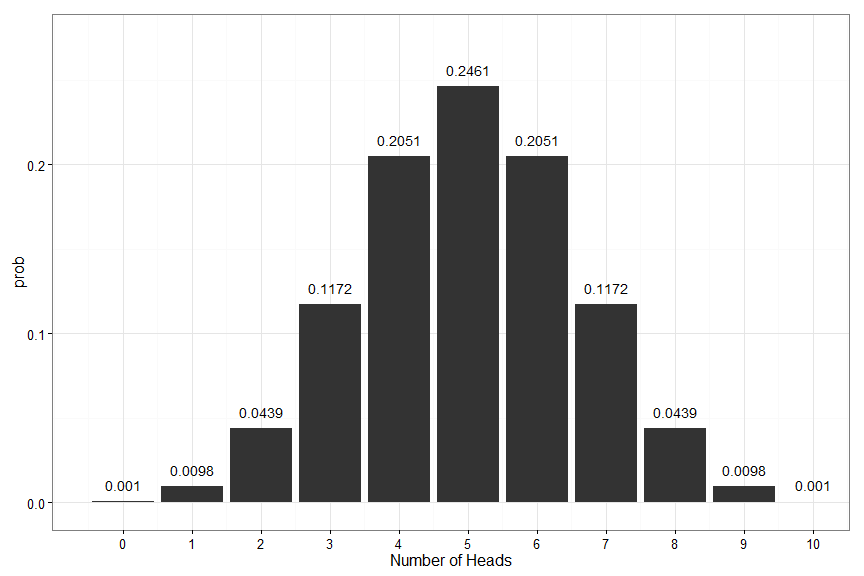
\includegraphics[width=3.5in]{figure/taste-1.png}
\caption{plot of chunk taste}
\end{figure}

\section{Taste Test Results}\label{taste-test-results-1}

\begin{itemize}
\itemsep1pt\parskip0pt\parsep0pt
\item
  If the taster cannot tell the difference, then there is a (roughly)
  17\% chance that she would get at least 7 correct in 10 trials
\item
  Something that happens 17 times out of 100 (17\% of the time) is not
  all that unusual (or unlikely)

  \begin{itemize}
  \itemsep1pt\parskip0pt\parsep0pt
  \item
    Depends on your definition of unusual (unlikely)
  \end{itemize}
\item
  In other words, if the taster cannot tell the difference, it is not
  all that unlikely that she would be able to get at least 7 correct on
  ten trials by randomly guessing
\item
  On the basis of this evidence, I do not have sufficient reason to
  reject the hypothesis that the taster can't tell the difference
\item
  I do not have sufficient evidence to conclude that the taster can tell
  the difference
\item
  The taster has failed to prove that she can tell the difference
\end{itemize}

\section{Taste Test: When can someone
tell?}\label{taste-test-when-can-someone-tell}

\begin{itemize}
\itemsep1pt\parskip0pt\parsep0pt
\item
  How many times would the taster have to get the correct answer in 10
  trials, in order to conclude that she can tell the difference?

  \begin{itemize}
  \itemsep1pt\parskip0pt\parsep0pt
  \item
    I would say, ``At least 8 out of 10''
  \item
    Because Pr(at least 8 correct in 10 trials) = 0.055
  \item
    If the taster can't tell the difference, then it would be unlikely
    (less than a 10\% chance) that she would be able to get at least 8
    correct by guessing
  \item
    10\% can be thought of as a lenient definition of unlikely
  \end{itemize}
\item
  Others may argue:

  \begin{itemize}
  \itemsep1pt\parskip0pt\parsep0pt
  \item
    You might say, ``At least 9 out of 10,'' because you consider
    something to be unlikely if the chance of it happening is less than
    5\%
  \item
    Someone else might say, ``10 out of 10,'' because he/she considers
    something to be unlikely if the chance of it happening is less than
    1\%
  \item
    1\% can be thought of as a stringent definition of unlikely
  \end{itemize}
\end{itemize}

\end{document}
